% !TEX root = ../OT4ML.tex

%%%%%%%%%%%%%%%%%%%%%%%%%%%%%%%%%%%%%%%%%%%%%%%%%%%%%%%%%%%%%%%%%%%%%%%%%%%
%%%%%%%%%%%%%%%%%%%%%%%%%%%%%%%%%%%%%%%%%%%%%%%%%%%%%%%%%%%%%%%%%%%%%%%%%%%
%%%%%%%%%%%%%%%%%%%%%%%%%%%%%%%%%%%%%%%%%%%%%%%%%%%%%%%%%%%%%%%%%%%%%%%%%%%
\section{Monge Problem between Measures}
\label{sec-monge}

The goal of this section is to pass from finite matching to transport between arbitrary probability laws. The central stakes are to define measures, push-forwards and Monge maps carefully enough that the discrete picture survives, while exposing why deterministic maps can fail to exist. Monge's original formulation~\cite{Monge1781} and modern treatments~\cite{Villani03,Villani09,SantambrogioBook,rachev1998mass} are the conceptual background for this transition.

The presentation of the previous section could only handle two sets with the same number of points. To relax this to a more general setting, one needs to consider probability distributions, so that the points are weighted by masses.

%%%%%%%%%%%%%%%%%%%%%%%%%%%%%%%%%%%%%%%%%%%%%%%%%%%%%%%%%%%%%%%%%%%%%%%%%%%
\subsection{Measures}
\label{sec-measures}

Measures are the language that lets point clouds, densities and singular objects be handled uniformly. We only recall the facts needed later: integration, total variation, densities and probabilistic laws.

%%%
\paragraph{Histograms}

We use the terms histogram and probability vector interchangeably for any element $\a \in \simplex_n$ of the probability simplex
\eq{
	\simplex_n \eqdef \enscond{\a \in \RR_+^n}{ \sum_{i=1}^n \a_i = 1 }.
}

%%%
\paragraph{Discrete measure, empirical measure}

A discrete measure with weights $\a$ and locations $x_1,\dots,x_n\in\X$ reads
\eql{\label{eq-discr-meas}
	\al = \sum_{i=1}^n \a_i \de_{x_i}
}
where $\de_x$ is the Dirac mass at position $x$, intuitively a unit of mass infinitely concentrated at location $x$. Such a measure is a probability measure if, additionally, $\a\in\simplex_n$, and more generally a positive measure if all weights $\a_i$ are nonnegative.
%
An ``empirical'' probability distribution is uniform on a point cloud, i.e. $\al=\frac{1}{n}\sum_i \de_{x_i}$.
%
In practice, in many applications, it is useful to be able to manipulate both the positions $x_i$ (``Lagrangian'' discretization) and the weights $\a_i$ (``Eulerian'' discretization). Lagrangian modification is usually more powerful (because it leads to adaptive discretization) but it breaks the convexity of most problems.


%%%%
\paragraph{General measures}

We consider Borel measures $\al \in \Mm(\X)$ on a metric space $(\Xx,d)$, meaning that $\al(A)$ is defined for every Borel set $A$ (obtained from open sets by countable unions, countable intersections and complements). Unless otherwise stated, the measures are finite.
%
A Dirac measure $\de_x$ is then defined as $\de_x(A)=1$ if $x \in A$ and $0$ otherwise, and this extends by linearity for discrete measures of the form~\eqref{eq-discr-meas} as
\eq{
	\al(A) = \sum_{x_i \in A} \a_i
}
%
We denote $\Mm_+(\X)$ the subset of all positive measures on $\X$, i.e. $\al(A) \geq 0$ (and $\al(\X)<+\infty$ for the measure to be finite). The set of probability measures is denoted $\Mm_+^1(\X)$, which means that any $\al \in \Mm_+^1(\X)$ is positive, and that $\al(\X)=1$.

\begin{defn}[Support of a measure]\label{def:support}
	The support $\supp(\al)$ of a Borel measure $\al$ on a metric space $\Xx$ is the smallest closed set of full $\al$-mass. Equivalently, $x\in\supp(\al)$ if every open ball centered at $x$ has positive $\al$-mass.
\end{defn}


%%%%
\paragraph{Radon measures}

Using Lebesgue integration, a Borel measure can be used to compute the integral of measurable functions (i.e. such that level sets $\enscond{x}{f(x) < t}$ are Borel sets), and we denote this pairing as
\eq{
	\dotp{f}{\al} \eqdef \int f(x) \d\al(x).
}
Integration of such a measurable $f$ against a discrete measure $\al$ computes a sum
\eq{
	\int_\X f(x) \d\al(x) = \sum_{i=1}^n \a_i f(x_i).
}


This applies in particular to continuous test functions, which are Borel measurable.
%
Integration against a finite measure on a compact space thus defines a continuous linear form $f \mapsto \int f \d\al$ on the Banach space of continuous functions $(\Cc(\Xx),\norm{\cdot}_\infty)$, indeed $|\int f \d\al| \leq \norm{f}_\infty |\al|(\Xx)$. On compact spaces, the converse is true: every continuous linear form on $\Cc(\Xx)$ is represented by integration against a finite signed Radon measure. This is the Riesz--Markov--Kakutani representation theorem~\cite{rudin1987realcomplex,bogachev2007measure}. It identifies $\Mm(\Xx)$ with the Banach dual of $\Cc(\Xx)$, and this duality pairing $\dotp{f}{\al}$ will be crucial for the convex duality arguments used later.

%%%%%
\paragraph{Relative densities.}

A measure $\al$ which is a weighting of another reference measure $\lambda$ is said to have a density, denoted $\d\al(x)=\density{\al}(x)\d\lambda(x)$, or $\density{\al}=\frac{\d\al}{\d\lambda}$. On $\RR^d$ the reference $\lambda$ is often Lebesgue measure $\d x$. This means that
\eq{
	\foralls h \in \Cc(\Xx), \quad
		\int_{\Xx} h(x) \d\al(x) = \int_{\Xx} h(x) \density{\al}(x) \d\lambda(x).
}

%%%%%
\paragraph{Total variation norm.}

The norm inherited from the duality $\Mm(\Xx)=\Cc(\Xx)^*$ is the total variation norm. We use the notation
\begin{defn}[Total variation]\label{defn-total-variation}
	For a finite signed Radon measure $\al$ on a compact space $\Xx$,
	\[
		\norm{\al}_{\TV}
		\eqdef
		\usup{f \in \Cc(\Xx)} \enscond{\dotp{f}{\al}}{\norm{f}_\infty \leq 1}.
	\]
\end{defn}
This formula is useful because it computes the norm of a measure as the operator norm of the corresponding linear form on $\Cc(\Xx)$.

The same norm also has a direct measure-theoretic expression. The absolute value of a signed measure is
\[
	|\al|(A)
	\eqdef
	\usup{A=\cup_i B_i} \sum_i |\al(B_i)|,
\]
where the supremum is over finite or countable measurable partitions of $A$. Thus, if $\al=\sum_i \a_i \de_{x_i}$ with distinct atoms, $|\al|=\sum_i |\a_i|\de_{x_i}$; if $\d\al(x)=\rho(x)\d\lambda(x)$, then $\d|\al|(x)=|\rho(x)|\d\lambda(x)$.

\begin{prop}[Dual and measure definitions of total variation]\label{prop-tv-dual-measure}
	For a finite signed Radon measure $\al$ on a compact space $\Xx$,
	\[
		\norm{\al}_{\TV}=|\al|(\Xx).
	\]
	Consequently $(\Mm(\Xx),\norm{\cdot}_{\TV})$ is isometrically the Banach dual of $(\Cc(\Xx),\norm{\cdot}_\infty)$.
\end{prop}
\begin{proof}
	The inequality $\norm{\al}_{\TV}\leq |\al|(\Xx)$ follows from
	\[
		\abs{\int f\,\d\al}\leq \int |f|\,\d|\al|\leq \norm{f}_\infty |\al|(\Xx).
	\]
	For the reverse inequality, write the Jordan decomposition $\al=\al^+-\al^-$, so that $|\al|=\al^++\al^-$. The measurable sign $s=\frac{\d\al}{\d|\al|}$ takes values in $\{-1,1\}$ outside a $|\al|$-null set and satisfies $\d\al=s\,\d|\al|$. By regularity of Radon measures on compact spaces, $s$ can be approximated in $L^1(|\al|)$ by continuous functions $f_k$ with $\norm{f_k}_\infty\leq1$. Hence $\int f_k\,\d\al\to\int s\,\d\al=|\al|(\Xx)$, which proves the equality. The final statement is the Riesz--Markov--Kakutani representation theorem with this norm.
\end{proof}

For two absolutely continuous measures $\d\al=\rho_\al\d\lambda$ and $\d\be=\rho_\be\d\lambda$, this gives the concrete formula
\[
	\norm{\al-\be}_{\TV}
	=
	\int_\Xx |\rho_\al(x)-\rho_\be(x)|\,\d\lambda(x).
\]
For two discrete measures written on the same union of supports, $\al=\sum_k a_k\delta_{z_k}$ and $\be=\sum_k b_k\delta_{z_k}$, with missing coefficients set to zero,
\[
	\norm{\al-\be}_{\TV}
	=
	\sum_k |a_k-b_k|.
\]
%%%%%
\paragraph{Probabilistic interpretation.}

Radon probability measures represent the laws of random variables. A random variable with values in $\X$ is a measurable map $X:\Omega\to\X$ from an abstract probability space $(\Omega,\PP)$. Its law is the Radon probability measure $\al$ defined by
\[
	\al(A)=\PP(\enscond{\omega\in\Omega}{X(\omega)\in A})
	\qquad\text{for Borel sets } A\subset \X .
\]
Integrals with respect to this law are expectations:
\[
	\int_\X f(x)\,\d\al(x)=\mathbb{E}[f(X)].
\]


%%%%%%%%%%%%%%%%%%%%%%%%%%%%%%%%%%%%%%%%%%%%%%%%%%%%%%%%%%%%%%%%%%%%%%%%%%%
\subsection{Push Forward}
\label{sec-push-forward}


Push-forwards encode how maps move mass. This short subsection is the bridge between deterministic maps and linear operations on measures.

For some continuous map $\T : \X \rightarrow \Y$, we define the pushforward operator $\T_\sharp : \Mm(\X) \rightarrow \Mm(\Y)$.
%
For a Dirac mass, one has $\T_\sharp \de_{x} = \de_{\T(x)}$, and this formula is extended to arbitrary measures by linearity. In some sense, moving from $\T$ to $\T_\sharp$ is a way to linearize any map at the price of moving from a (possibly) finite-dimensional space $\Xx$ to the infinite-dimensional space $\Mm(\Xx)$, and this idea is central to many convex relaxation methods, most notably Lasserre's relaxation.
%
For discrete measures~\eqref{eq-discr-meas}, the pushforward operation consists simply in moving the positions of all the points in the support of the measure
\eq{
	\T_{\sharp} \al \eqdef \sum_i \a_i \de_{\T(x_i)}.
}
For more general measures, for instance for those with a density, the notion of push-forward plays a fundamental role in describing spatial modifications of probability measures. The formal definition reads as follows.

\begin{defn}[Push-forward]\label{defn-pushfwd}
For $\T : \X \rightarrow \Y$, the push forward measure $\be = \T_\sharp \al \in \Mm(\Y)$ of some $\al \in \Mm(\X)$ satisfies
\eql{\label{eq-push-fwd}
	\foralls h \in \Cc(\Y), \quad \int_\Y h(y) \d \be(y) = \int_\X h(\T(x)) \d\al(x).
}
Equivalently, for any measurable set $B \subset \Y$, one has
\eql{\label{eq-equiv-pushfwd}
	\be(B) = \al( \enscond{x \in \X}{\T(x) \in B} ).
}
Note that $\T_\sharp$ preserves positivity and total mass, so that if $\al \in \Mm_+^1(\X)$ then $\T_\sharp \al \in \Mm_+^1(\Y)$.
\end{defn}


%%%%%%%
\begin{prop}[Push-forward formula for densities]\label{prop-push-forward-densities}
	Let $\alpha$ and $\beta$ have densities $\density{\al}$ and $\density{\be}$ on open subsets of $\RR^\dims$. Assume that $T$ is a $C^1$ diffeomorphism and that $\beta=T_\sharp\alpha$. Then, for all $x$,
	\eql{\label{eq-pfwd-density}
			\density{\al}(x) = |\det(\T'(x))| \density{\be}(\T(x)).
	}
	Equivalently, for $y=T(x)$,
	\[
		\rho_\beta(y)=\rho_\alpha(T^{-1}y)\,
		\frac{1}{|\det T'(T^{-1}y)|}.
	\]
\end{prop}

\begin{proof}
Explicitly doing the change of variable $y=T(x)$, so that $\d y = |\det(T'(x))| \d x$ in formula~\eqref{eq-push-fwd} for measures with densities $(\density{\al},\density{\be})$ on $\RR^\dims$ (assuming $\T$ is smooth and a bijection), one has for all $h \in \Cc(\Yy)$
\begin{align*}
	\int_\Yy h(y)\rho_\be(y) \d y &= \int_\Yy h(y) \d \be(y) = \int_\Xx h(T(x)) \d \al(x) = \int_\Xx h(T(x)) \rho_\al(x) \d x \\
		&= \int_\Yy h(y) \rho_\al(T^{-1}y) \frac{\d y}{|\det(T'( T^{-1} y))|},
\end{align*}
which shows that
\eq{
	\rho_\be(y) = \rho_\al(T^{-1}y) \frac{1}{|\det(T'( T^{-1} y))|}.
}
Since $T$ is a diffeomorphism, one obtains equivalently
\eq{
		\density{\al}(x) = |\det(\T'(x))| \density{\be}(\T(x))
}
where $\T'(x) \in \RR^{\dims \times \dims}$ is the Jacobian matrix of $T$ (the matrix formed by taking the gradient of each coordinate of $T$).
%
This implies, denoting $y=\T(x)$
\eq{
	|\det(\T'(x))| = \frac{ \density{\al}(x) }{ \density{\be}(y) }.
}
\end{proof}
%%%%%%%


\begin{rem}[Probabilistic interpretation]
The law, i.e. probability distribution, of a random variable $X$ is the push-forward of $\PP$ by $X$, namely $\al=X_\sharp\PP$.
%
Applying another push-forward $\be = \T_\sharp\al$ for $\T : \X \rightarrow \Y$, following~\eqref{eq-push-fwd}, is equivalent to defining another random variable $Y=\T(X)$, namely $\omega \in \Om \mapsto \T(X(\omega)) \in \Y$. Thus $\be$ is the law of $Y$.
%
Drawing a random sample $y$ from $Y$ is thus simply achieved by computing $y=\T(x)$ where $x$ is drawn from $X$.
\end{rem}

%%%%%%%%%%%%%%%%%%%%%%%%%%%%%%%%%%%%%%%%%%%%%%%%%%%%%%%%%%%%%%%%%%%%%%%%%%%
\subsection{Monge's Formulation}
\label{sec-monge-formulation}
\label{sec-continuous-monge}

Monge's problem asks for a deterministic map transporting one law onto another while minimizing a prescribed cost. This is the original formulation introduced by Monge in his memoir on the ``d\'eblai et remblai'' problem~\cite{Monge1781}. It is geometrically direct, because every source point is assigned one destination, but it is also analytically fragile: the feasible set is non-convex, it can be empty, and a map cannot split mass. These limitations are precisely what motivate Kantorovich's relaxation in the next section.

\paragraph{Monge problem.}

Given $\al\in\Mm_+^1(\Xx)$, $\be\in\Mm_+^1(\Yy)$ and a cost $c:\Xx\times\Yy\to\RR_+$, the Monge problem is
\eql{\label{eq-monge-continuous}
	\Monge_c(\al,\be)
	\eqdef
	\inf_{\T:\Xx\to\Yy}
	\enscond{\int_\Xx c(x,\T(x))\d\al(x)}{\T_\sharp\al=\be}.
}
The constraint $\T_\sharp\al=\be$ means that $\T$ pushes the mass of $\al$ onto $\be$ in the sense of Definition~\ref{defn-pushfwd}.

\begin{prop}[Empirical Monge maps and matchings]\label{prop-empirical-monge-matching}
	Assume that the source atoms $x_1,\ldots,x_n$ are distinct and that
	\[
		\al=\frac1n\sum_{i=1}^n\de_{x_i},
		\qquad
		\be=\frac1n\sum_{j=1}^n\de_{y_j}.
	\]
	If $\T_\sharp\al=\be$, then for each distinct target value $z$ in the support of $\be$, exactly $n\be(\{z\})$ source atoms are mapped to $z$. In particular, if the $y_j$ are distinct, then there exists a permutation $\sigma\in\Perm(n)$ such that $\T(x_i)=y_{\sigma(i)}$ for all $i$. Conversely, every such assignment of source atoms to target atoms with the correct masses defines a feasible Monge map on the support of $\al$, and in the distinct-target case
	\[
		\int_\Xx c(x,\T(x))\d\al(x)=\frac1n\sum_{i=1}^n c(x_i,y_{\sigma(i)}).
	\]
	If source locations are repeated, they should first be merged into atoms with larger masses; such atoms cannot be split by a Monge map.
\end{prop}
\begin{proof}
	Since $\T_\sharp\al=\be$, all images $\T(x_i)$ must belong to the support of $\be$; otherwise the push-forward would give positive mass to a point outside that support. For any target atom $z$,
	\[
		\be(\{z\})=\al(\T^{-1}(\{z\}))=\frac1n\#\enscond{i}{\T(x_i)=z}.
	\]
	This proves the counting statement. If all target atoms have mass $1/n$, each target receives exactly one source atom, which is a permutation. The converse and the cost identity follow by direct substitution.
\end{proof}

\begin{prop}[Existence of transport maps from atomless sources]\label{prop-existence-transport-map-atomless}
	Let $\al$ and $\be$ be Borel probability measures on Polish spaces, and assume that $\al$ is atomless. Then there exists a measurable map $\T$ such that $\T_\sharp\al=\be$.
\end{prop}
\begin{proof}
	A standard measure-isomorphism theorem identifies the atomless probability space generated by $\al$ with Lebesgue measure on $[0,1]$, modulo null sets~\cite{bogachev2007measure}. It is therefore enough to construct a map from $[0,1]$ to the target law $\be$. Choose a Borel isomorphism $i$ from the support of $\be$ onto a Borel subset of $[0,1]$, set $\nu=i_\sharp\be$, and use the generalized inverse of the cumulative distribution function of $\nu$. This map sends Lebesgue measure on $[0,1]$ to $\nu$ and takes values in $i(\supp\be)$ almost surely. Composing with $i^{-1}$ and then with the source isomorphism gives a measurable transport map from $\al$ to $\be$.
\end{proof}

\begin{rem}[Feasibility versus optimality]
	An optimal map solving~\eqref{eq-monge-continuous} might fail to exist for two distinct reasons. First, the constraint set can be empty, for instance if $\al=\de_x$ and $\be$ is not a single Dirac mass. Proposition~\ref{prop-existence-transport-map-atomless} shows that non-atomicity of the source removes this feasibility obstruction. Second, even when feasible maps exist, the infimum may fail to be attained because the class of maps is not closed under weak limits.
\end{rem}

\begin{example}[A splitting obstruction]\label{ex-splitting-obstruction}
	A classical example, discussed for instance in~\cite{SantambrogioBook}, takes $\al$ uniform on a vertical segment and $\be$ equal to the average of the uniform measures on two parallel vertical segments placed symmetrically to the left and to the right. For the quadratic cost, the relaxed Kantorovich optimizer splits each source point into its two symmetric targets. A deterministic Monge map cannot split one point into two destinations, so minimizing sequences must oscillate between the two sides and the Monge problem has no optimizer.
\end{example}

\begin{example}[Semi-discrete Monge maps]
	The Monge formulation is not symmetric in $\al$ and $\be$. It makes sense, for instance, when $\al$ has a density with respect to Lebesgue measure and $\be$ is discrete. On $\Xx=\Yy=\RR^d$, let $\be=\sum_j b_j\delta_{y_j}$ be supported on $\{y_1,\ldots,y_m\}$. A map $\T$ such that $\T_\sharp\al=\be$ defines a segmentation of the space into cells
	\[
		C_j\eqdef \T^{-1}(y_j),
		\qquad
		\al(C_j)=b_j.
	\]
	This is the semi-discrete setting. Section~\ref{sec-semidiscr-w1} explains how the cells become Laguerre cells for prescribed masses and ordinary Voronoi cells when the masses are free. If one exchanges the roles of $\al$ and $\be$ so that $\al$ is discrete, then no valid $\T$ exists in general: it is not possible to push forward a discrete measure to a measure with density.
\end{example}

Figure~\ref{fig:monge-color-transfer-rgb} shows a finite-dimensional instance of this deterministic viewpoint. The source and target measures are empirical color clouds in RGB space, and the map transports colors while leaving pixel positions fixed.

\begin{figure}[H]
\centering
\begin{tabular}{@{}ccccc@{}}
\small source & \small $t=1/3$ & \small $t=2/3$ & \small transported & \small target \\[-.15em]
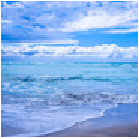
\includegraphics[width=.17\linewidth]{figures/monge-color-transfer-rgb/image-t000.pdf} &

\includegraphics[width=.17\linewidth]{figures/monge-color-transfer-rgb/image-t033.pdf} &

\includegraphics[width=.17\linewidth]{figures/monge-color-transfer-rgb/image-t067.pdf} &

\includegraphics[width=.17\linewidth]{figures/monge-color-transfer-rgb/image-t100.pdf} &

\includegraphics[width=.17\linewidth]{figures/monge-color-transfer-rgb/image-target.pdf} \\[-.1em]

\includegraphics[width=.17\linewidth]{figures/monge-color-transfer-rgb/rgb-t000.pdf} &

\includegraphics[width=.17\linewidth]{figures/monge-color-transfer-rgb/rgb-t033.pdf} &

\includegraphics[width=.17\linewidth]{figures/monge-color-transfer-rgb/rgb-t067.pdf} &
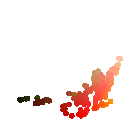
\includegraphics[width=.17\linewidth]{figures/monge-color-transfer-rgb/rgb-t100.pdf} &
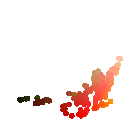
\includegraphics[width=.17\linewidth]{figures/monge-color-transfer-rgb/rgb-target.pdf}
\end{tabular}
\caption{Color transfer as a Monge map in RGB space, from a beach photograph to a flower photograph. The top row applies the palette map to the source image; the bottom row shows the empirical color clouds in the RGB cube. Only colors are transported here, not pixel locations.}
\label{fig:monge-color-transfer-rgb}
\end{figure}

\paragraph{Monge distance.}

When $\Xx=\Yy$ and $c(x,y)=d(x,y)^p$ for a metric $d$, set
\[
	\Ee_\al(\T)
	\eqdef
	\int_\Xx d(x,\T(x))^p\d\al(x).
\]
The Monge value defines the directed quantity
\eql{\label{eq-monge-distance}
	\tilde\Wass_p(\al,\be)^p
	\eqdef
	\inf_{\T:\Xx\to\Xx}
	\enscond{\Ee_\al(\T)}{\T_\sharp\al=\be}.
}
If the constraint set is empty, then $\tilde\Wass_p(\al,\be)=+\infty$.

\begin{prop}[Directed Monge distance]\label{prop-directed-monge-distance}
	Assume that $\Xx=\Yy$ is a compact metric space. The quantity $\tilde\Wass_p$ is nonnegative, vanishes only on the diagonal, and satisfies the triangle inequality. It is therefore a directed extended distance: it need not be symmetric and may take the value $+\infty$.
\end{prop}
\begin{proof}
	Nonnegativity is immediate. If $\tilde\Wass_p(\al,\be)=0$, choose feasible maps $\T_k$ with $\int d(x,\T_k(x))^p\d\al(x)\to0$. For every continuous function $h$, compactness gives uniform continuity, hence
	\[
		\left|\int h\d\be-\int h\d\al\right|
		=
		\left|\int h(\T_k(x))-h(x)\d\al(x)\right|
		\longrightarrow0.
	\]
	Thus $\al=\be$.

	We prove the triangle inequality. If $\tilde\Wass_p(\al,\be)=+\infty$ while both $\tilde\Wass_p(\al,\ga)$ and $\tilde\Wass_p(\ga,\be)$ were finite, there would be maps $S_\sharp\al=\ga$ and $T_\sharp\ga=\be$, hence $(T\circ S)_\sharp\al=\be$, a contradiction. Thus the inequality is automatic whenever the left-hand side is infinite. In the finite case, fix $\epsilon>0$ and choose $\epsilon$-minimizers $S_\sharp\al=\ga$ and $T_\sharp\ga=\be$ such that
	\[
		\Ee_\al(S)^{1/p}\leq\tilde\Wass_p(\al,\ga)+\epsilon,
		\qquad
		\Ee_\ga(T)^{1/p}\leq\tilde\Wass_p(\ga,\be)+\epsilon.
	\]
	The composed map is feasible from $\al$ to $\be$, and Minkowski's inequality gives
	\[
	\begin{aligned}
		\tilde\Wass_p(\al,\be)
		&\leq
		\left(\int d(x,T(S(x)))^p\d\al(x)\right)^{1/p} \\
		&\leq
		\left(\int d(x,S(x))^p\d\al(x)\right)^{1/p}
		+
		\left(\int d(S(x),T(S(x)))^p\d\al(x)\right)^{1/p} \\
		&=
		\Ee_\al(S)^{1/p}+\Ee_\ga(T)^{1/p}
		\leq
		\tilde\Wass_p(\al,\ga)+\tilde\Wass_p(\ga,\be)+2\epsilon.
	\end{aligned}
	\]
	Letting $\epsilon\to0$ gives the result.
\end{proof}

The directed value $\tilde\Wass_p$ is useful conceptually, but it is too rigid to be the main distance between measures: it can be infinite and asymmetric. The Kantorovich formulation remedies both issues by replacing maps with couplings.

%%%%%%%%%%%%%%%%%%%%%%%%%%%%%%%%%%%%%%%%%%%%%%%%%%%%%%%%%%%%%%%%%%%%%%%%%%%
\subsection{Existence and Uniqueness of the Monge Map}
\label{sec-monge-existence-uniqueness}

This subsection records the main regimes where Monge's deterministic formulation becomes well posed. Brenier's theorem is the central result: for the squared Euclidean cost, absolute continuity of the source restores existence, uniqueness and convex-potential structure.

\paragraph{Brenier's theorem.}

Brenier's theorem~\cite{MR923203,Brenier91} ensures that, in $\RR^d$ for the quadratic cost, absolute continuity of the source is enough for Monge's problem to have a unique solution. It also gives the decisive structural description of this solution: the optimal map is not an arbitrary map, but the gradient of a convex potential.

\begin{thm}[Brenier]\label{thm-brenier}
	Let $\al,\be\in\Mm_+^1(\RR^d)$ have finite second moments, and assume that $\al$ is absolutely continuous with respect to Lebesgue measure. For the quadratic cost $c(x,y)=\norm{x-y}^2$, there exists a convex function $\phi:\RR^d\to\RR\cup\{+\infty\}$ such that
	\[
		\T=\nabla\phi,
		\qquad
		\T_\sharp\al=\be,
	\]
	and $\T$ is the unique optimal Monge map $\al$-almost everywhere. The optimal Kantorovich plan is $(\Id,\T)_\sharp\al$.
\end{thm}
\begin{proof}
	The proof uses the Kantorovich relaxation and duality developed later in Section~\ref{sec-dual}. Kantorovich duality for the quadratic cost gives optimal potentials $(f,g)$ with equality $f(x)+g(y)=\norm{x-y}^2$ on the support of any optimal plan. After subtracting the harmless quadratic terms, this equality is equivalent to the Fenchel equality $\phi(x)+\phi^*(y)=\dotp{x}{y}$ for a convex function $\phi$. Hence the support of every optimal plan lies in the graph of the subdifferential $\partial\phi$. Since $\al$ has a density and convex functions are differentiable Lebesgue-almost everywhere, $\partial\phi(x)$ is a singleton for $\al$-almost every $x$. The plan is therefore concentrated on the graph of $\T=\nabla\phi$, which proves that the relaxed optimizer is induced by a Monge map. Any two optimal plans are concentrated on the same single-valued graph $\al$-almost everywhere, which gives uniqueness of the map. This is the standard route behind Brenier's polar factorization theorem; related existence and uniqueness results for more general strictly convex costs are developed for instance in~\cite{gangbo1996geometry,caffarelli2002constructing,Villani09}.
\end{proof}

\begin{defn}[Measures not charging hypersurfaces]\label{defn-not-charging-hypersurfaces}
	A Borel measure $\al$ on $\RR^d$ does not charge hypersurfaces if $\al(S)=0$ for every countably $(d-1)$-rectifiable set $S$, i.e. every set that can be covered, up to an $\mathcal H^{d-1}$-null set, by countably many $C^1$ hypersurfaces.
\end{defn}

\begin{rem}[A sharp source hypothesis]
	The absolute-continuity assumption in Brenier's theorem can be weakened: for the quadratic cost, it is enough that $\al$ does not charge hypersurfaces~\cite{gangbo1996geometry,Villani09,SantambrogioBook}. The reason is that the set where a convex potential has a genuinely multi-valued subdifferential is contained in a countable union of lower-dimensional pieces. This condition is close to sharp. If the source gives positive mass to a segment or a hypersurface, the subdifferential may be multi-valued on a set of positive $\al$-mass, and the optimal relaxed plan may need to split mass, as in Example~\ref{ex-splitting-obstruction}.
\end{rem}

\begin{rem}[Beyond the quadratic Euclidean cost]
	Brenier's theorem is the cleanest statement because the squared Euclidean cost turns optimal maps into gradients of convex functions. For costs $c(x,y)=\norm{x-y}^p$ with $p>1$, or more generally costs $c(x,y)=h(x-y)$ with $h$ smooth and strictly convex, the same strategy gives a unique optimal map under absolute continuity of the source, but the map is written in terms of a $c$-convex potential. On a Riemannian manifold, the local analogue for the cost $d_M(x,y)^2/2$ uses the exponential map
	\[
		\T(x)=\exp_x(-\nabla\phi(x)),
	\]
	where $\phi$ is $c$-convex. The main additional issues are the cut locus and regularity of geodesics, which is why the Euclidean statement is usually presented first. These extensions are part of McCann's displacement convexity theory and the general theory of optimal maps on manifolds~\cite{mccann1997convexity,Villani09}.
\end{rem}

Brenier's theorem should be understood through the analogy between convex gradients and increasing functions. The gradient of a convex function is a monotone field:
\[
	\dotp{\nabla\phi(x)-\nabla\phi(x')}{x-x'}\geq0.
\]

\begin{rem}[Monotone fields need not be gradients]
	In dimensions larger than one, not all monotone fields are gradients of convex functions. Consider in $\RR^2$ the rotation matrix
	\[
		R_\theta=\begin{pmatrix}
		\cos\theta & -\sin\theta\\
		\sin\theta & \cos\theta
		\end{pmatrix}.
	\]
	The linear map $x\mapsto R_\theta x$ is monotone as soon as $|\theta|\leq\pi/2$, because
	\[
		\dotp{R_\theta x-R_\theta x'}{x-x'}
		=
		\dotp{R_\theta(x-x')}{x-x'}
		=
		\cos(\theta)\norm{x-x'}^2\geq0.
	\]
	However, for $\theta\neq0$, $R_\theta$ is not symmetric and therefore cannot be the gradient of a scalar potential. Indeed, if a linear field $Ax$ equals $\nabla\phi(x)$, then its Jacobian $A$ must be symmetric; equivalently, a quadratic potential $\phi(x)=\dotp{Bx}{x}/2$ has gradient $((B+B^\top)/2)x$. Thus monotonicity is weaker than Brenier optimality in dimension $d\geq2$.
\end{rem}

McCann's displacement convexity theory clarifies the geometric meaning of interpolating along Brenier maps~\cite{mccann1997convexity}; this is the language of Wasserstein geodesics used later for barycenters in Section~\ref{sec-barycenters} and for gradient flows in Section~\ref{sec-wasserstein-gradient-flows}. Caffarelli's regularity theory, discussed next, explains when the convex potential is actually smooth enough to define a classical deformation.

\begin{prop}[Polar factorization]\label{prop-polar-factorization}
	Let $\Omega\subset\RR^d$ be endowed with normalized Lebesgue measure $\lambda$, and let $u\in L^2(\Omega;\RR^d)$. Assume that the law $\nu=u_\sharp\lambda$ has finite second moment. Then there exist a measure-preserving map $s:\Omega\to\Omega$ and a convex function $\phi$ such that
	\[
		u=\nabla\phi\circ s
		\qquad \lambda\text{-a.e.}
	\]
	The Brenier factor $\nabla\phi$ is unique $\lambda$-almost everywhere.
\end{prop}
\begin{proof}
	By Brenier's theorem there is a unique gradient of a convex function $\T=\nabla\phi$ transporting $\lambda$ to $\nu$. The maps $u$ and $\T$ have the same image law. The rearrangement theorem for non-atomic probability spaces gives a measure-preserving map $s$ such that $u=\T\circ s$; equivalently, $s$ chooses, with the correct conditional probabilities, preimages of $u(x)$ under $\T$. Uniqueness of the Brenier factor follows from Theorem~\ref{thm-brenier}. In the Gaussian linear case, with reference $\Gaussian(0,\Id)$ and $u(x)=Ax$, this is the usual matrix polar decomposition: $A=SO$ with $S=(AA^\top)^{1/2}$ symmetric positive semidefinite, $Sx$ is the Brenier part and $Ox$ is measure preserving.
\end{proof}

\paragraph{Regularity and the Monge--Amp\`ere equation.}

\begin{prop}[Caffarelli regularity]\label{prop-caffarelli-regularity}
	Let $\Omega,\Lambda\subset\RR^d$ be bounded uniformly convex domains with $C^2$ boundaries. Let $\al=\rho(x)\d x$ be supported on $\Omega$ and $\be=\eta(y)\d y$ be supported on $\Lambda$, with $0<m\leq\rho,\eta\leq M<+\infty$. If $\rho,\eta\in C^\alpha$ for some $\alpha\in(0,1)$, then the Brenier potential $\phi$ transporting $\al$ to $\be$ is strictly convex and satisfies $\phi\in C^{2,\alpha}_{\mathrm{loc}}(\Omega)$; in particular $\nabla\phi$ is locally H\"older. Under the corresponding boundary compatibility and smoothness assumptions, the regularity holds up to the boundary.
\end{prop}
\begin{proof}
	The potential solves the Monge--Amp\`ere equation
	\[
		\det(\nabla^2\phi(x))
		=
		\frac{\rho(x)}{\eta(\nabla\phi(x))}
	\]
	in the Alexandrov sense, with second boundary condition $\nabla\phi(\Omega)=\Lambda$. The density bounds and convexity of the domains give strict convexity and localization of sections. Caffarelli's interior theory then yields $C^{2,\alpha}_{\mathrm{loc}}$ estimates for $\phi$; the boundary statement follows from the boundary regularity theory under uniform convexity and compatibility assumptions~\cite{caffarelli2003monge,Villani09}.
\end{proof}

\begin{rem}[Regularity, weak maps, and splitting]
	Caffarelli's theorem should be read as a warning as well as a theorem. Brenier's theorem gives existence and uniqueness under mild assumptions, but smoothness requires density bounds, smoothness and convex geometry that are rarely satisfied by empirical, manifold-supported or neural generative distributions. In such applications, the exact OT map is often only weakly defined, possibly unstable, and better represented by a coupling, an entropic approximation or a learned parametric surrogate.

	Even without smoothness, the convex potential is locally Lipschitz on the interior of its domain, so $\nabla\phi$ is defined Lebesgue-almost everywhere. If the source measure does not satisfy the non-splitting hypotheses of Brenier's theorem, the correct relaxed object is instead an optimal Kantorovich plan concentrated on the graph of the set-valued map $\partial\phi$. At points where $\partial\phi(x)$ contains several target locations, the plan may split the mass starting from $x$. Thus the subdifferential still describes the geometry of optimality, but the transport object is a coupling rather than a single-valued map.
\end{rem}

For smooth densities, the change-of-variables formula~\eqref{eq-pfwd-density} gives the Monge--Amp\`ere equation
\eql{\label{eq-monge-ampere}
	\det(\nabla^2\phi(x))\density{\be}(\nabla\phi(x))=\density{\al}(x).
}
With suitable boundary conditions, this characterizes the Brenier potential up to an additive constant among convex solutions. The convexity constraint forces $\det(\nabla^2\phi(x))\geq0$ and is necessary for this fully nonlinear elliptic equation to be well posed. Numerical schemes for this PDE connect OT with fully nonlinear elliptic solvers; see for instance~\cite{Benamou:2014jw,froese2011convergent}.

The Monge--Amp\`ere operator can be viewed as a nonlinear degenerate analogue of the Laplacian. To see this, write
\[
	\phi(x)=\frac{\norm{x}^2}{2}+\epsilon\psi(x),
	\qquad
	\T(x)=\nabla\phi(x)=x+\epsilon\nabla\psi(x).
\]
Writing the densities of $\al$ and $\be$ as $\rho_\al$ and $\rho_\be$, the density equation becomes
\[
	\rho_\al(x)
	=
	\det(I+\epsilon\nabla^2\psi(x))\,
	\rho_\be(x+\epsilon\nabla\psi(x)).
\]
Using $\det(I+\epsilon A)=1+\epsilon\tr(A)+o(\epsilon)$ and Taylor expanding $\rho_\be$ gives
\[
	\rho_\al
	=
	\rho_\be
	+\epsilon\bigl(\rho_\be\Delta\psi+\dotp{\nabla\rho_\be}{\nabla\psi}\bigr)
	+o(\epsilon)
	=
	\rho_\be+\epsilon\nabla\cdot(\rho_\be\nabla\psi)+o(\epsilon).
\]
Thus, if both densities are perturbations of a common smooth density $\rho$ and $\rho_\be-\rho_\al=\epsilon\eta+o(\epsilon)$, the first-order equation is the weighted Poisson equation $-\nabla\cdot(\rho\nabla\psi)=\eta$. The following proposition records the same linearization in reference-measure form.

\begin{prop}[Linearization of the Monge--Amp\`ere equation]\label{prop-linearized-monge-ampere}
	Let $\rho_\epsilon=\rho_0+\epsilon r+o(\epsilon)$ be a smooth perturbation of a positive reference density $\rho_0$ on a smooth bounded domain, with $\int r=0$. If $\T_\epsilon(x)=x+\epsilon\nabla u(x)+o(\epsilon)$ transports $\rho_0$ to $\rho_\epsilon$, then, to first order,
	\[
		-\nabla\cdot(\rho_0\nabla u)=r.
	\]
	In particular, when $\rho_0$ is constant, the linearized equation is $-\Delta u=r/\rho_0$.
\end{prop}
\begin{proof}
	The change-of-variables equation for $\T_\epsilon$ is
	\[
		\rho_0(x)
		=
		\rho_\epsilon(\T_\epsilon(x))\det(\nabla \T_\epsilon(x)).
	\]
	Expanding $\rho_\epsilon(x+\epsilon\nabla u)=\rho_0(x)+\epsilon r(x)+\epsilon\dotp{\nabla\rho_0}{\nabla u}+o(\epsilon)$ and
	\[
		\det(I+\epsilon\nabla^2u)=1+\epsilon\Delta u+o(\epsilon)
	\]
	gives
	\[
		\rho_0
		=
		\rho_0+
		\epsilon\bigl(r+\dotp{\nabla\rho_0}{\nabla u}+\rho_0\Delta u\bigr)+o(\epsilon)
		=
		\rho_0+
		\epsilon\bigl(r+\nabla\cdot(\rho_0\nabla u)\bigr)+o(\epsilon).
	\]
	The first-order term must vanish.
\end{proof}

%%%%%%%%%%%%%%%%%%%%%%%%%%%%%%%%%%%%%%%%%%%%%%%%%%%%%%%%%%%%%%%%%%%%%%%%%%%
\subsection{One-Dimensional Transport and Quantiles}
\label{sec-1d-transport-quantiles}

In one dimension, optimal transport is completely explicit. The cumulative distribution function orders the mass, and the optimal coupling is obtained by matching equal quantile levels. This special case is both a computational tool and the template for several linearized constructions used later.

\begin{defn}[Cumulative and quantile functions]\label{def-cdf-quantile}
	For $\al\in\Mm_+^1(\RR)$, its cumulative distribution function is
	\eql{\label{eq-cumul-defn}
		\cumul{\al}(x)\eqdef\al((-\infty,x]).
	}
	Its generalized inverse, or quantile function, is
	\eql{\label{eq-OT-map-1d}
		\cumul{\al}^{-1}(r)
		\eqdef
		\inf\enscond{x\in\RR}{\cumul{\al}(x)\geq r},
		\qquad r\in(0,1).
	}
\end{defn}

\begin{prop}[Quantile push-forward]\label{prop-quantile-pushforward}
	One has $(\cumul{\al}^{-1})_\sharp\mathrm{Leb}_{[0,1]}=\al$. If $\al$ has no atoms, then $(\cumul{\al})_\sharp\al=\mathrm{Leb}_{[0,1]}$.
\end{prop}
\begin{proof}
	For simplicity, assume first that $\al$ has a strictly positive density, so that $\cumul{\al}$ is strictly increasing and continuous. Denote $\ga\eqdef(\cumul{\al}^{-1})_\sharp\mathrm{Leb}_{[0,1]}$. It is enough to prove that $\cumul{\ga}=\cumul{\al}$. For every $x$,
	\[
	\begin{aligned}
		\cumul{\ga}(x)
		&=
		\int_0^1 \mathbf 1_{(-\infty,x]}(\cumul{\al}^{-1}(z))\d z
		=
		\int_0^1 \mathbf 1_{[0,\cumul{\al}(x)]}(z)\d z
		=
		\cumul{\al}(x),
	\end{aligned}
	\]
	where we used $\cumul{\al}^{-1}(z)\leq x$ if and only if $z\leq\cumul{\al}(x)$. General measures follow from the same argument with generalized inverses and right-continuity of the cumulative distribution function. If $\al$ has no atoms, the probability integral transform gives $(\cumul{\al})_\sharp\al=\mathrm{Leb}_{[0,1]}$.
\end{proof}

If $\al$ has no atoms, the map
\eql{\label{eq-1d-monge-map}
	\T=\cumul{\be}^{-1}\circ\cumul{\al}
}
satisfies $\T_\sharp\al=\be$.

For the cost $c(x,y)=|x-y|^2$, this map is nondecreasing, hence the derivative of a convex function in dimension one. Brenier's theorem therefore identifies it as the optimal Monge map whenever $\al$ is atomless. With generalized inverses, the same quantile construction gives the optimal Kantorovich coupling for arbitrary measures, and it is also optimal for costs of the form $h(|x-y|)$ with $h$ convex and nondecreasing.

\begin{prop}[Monotone rearrangement on the line]\label{prop-1d-quantile-map}
	Let $\al,\be\in\Mm_+^1(\RR)$ have finite $p$-th moments, with $p\geq1$. The coupling
	\[
		\pi^\star=(\cumul{\al}^{-1},\cumul{\be}^{-1})_\sharp\mathrm{Leb}_{[0,1]}
	\]
	minimizes $\int |x-y|^p\d\pi(x,y)$ among couplings. If $\al$ has no atoms, it is induced by the monotone Monge map~\eqref{eq-1d-monge-map}.
\end{prop}
\begin{proof}
	The displayed measure is a coupling by Proposition~\ref{prop-quantile-pushforward}. Its support is monotone: for $s<t$, both quantile functions satisfy $\cumul{\al}^{-1}(s)\leq\cumul{\al}^{-1}(t)$ and $\cumul{\be}^{-1}(s)\leq\cumul{\be}^{-1}(t)$. If a coupling had two crossed pairs $x<x'$ and $y>y'$ with positive mass, exchanging the targets decreases the cost for strictly convex powers and does not increase it for $p=1$, by the two-point inequality used in Proposition~\ref{prop-matching-1d-monotone}. Eliminating crossings yields a monotone optimal coupling, and the monotone coupling with prescribed marginals is exactly the quantile coupling. If $\al$ has no atoms, $(\cumul{\al})_\sharp\al=\mathrm{Leb}_{[0,1]}$, so the coupling is generated by~\eqref{eq-1d-monge-map}.
\end{proof}

For discrete measures, one cannot directly apply the map formula when the source has atoms, but if the measures are uniform on the same number of Dirac masses, then it is exactly the sorting formula of Proposition~\ref{prop-matching-1d-monotone}.

\begin{prop}[One-dimensional Wasserstein formulas]\label{prop-wass-quantile-1d}
	Let $\al,\be\in\Mm_+^1(\RR)$ have finite $p$-th moments. For every $p\geq1$,
	\eql{\label{eq-wass-cumul}
		\Wass_p(\al,\be)^p
		=
		\int_0^1\abs{\cumul{\al}^{-1}(r)-\cumul{\be}^{-1}(r)}^p\d r
		=
		\norm{\cumul{\al}^{-1}-\cumul{\be}^{-1}}_{L^p([0,1])}^p.
	}
	For $p=1$, this is equivalently
	\begin{align}\label{eq-w1-1d}
		\Wass_1(\al,\be)
		&=
		\norm{\cumul{\al}-\cumul{\be}}_{L^1(\RR)}
		=
		\int_\RR \abs{\cumul{\al}(x)-\cumul{\be}(x)}\d x \\
		&=
		\int_\RR \abs{\int_{-\infty}^x\d(\al-\be)}\d x.
	\end{align}
\end{prop}
\begin{proof}
	The first formula follows from Proposition~\ref{prop-1d-quantile-map}: the optimal coupling is obtained by taking the same quantile level $r$ for both measures. For $p=1$, use the layer-cake identity. If $q_\al$ and $q_\be$ are the two quantile functions, then
	\[
		\int_0^1 |q_\al(r)-q_\be(r)|\d r
		=
		\int_\RR
		\lambda\bigl(\{r:q_\al(r)\leq x<q_\be(r)\}\cup\{r:q_\be(r)\leq x<q_\al(r)\}\bigr)\d x.
	\]
	The measure of the displayed set is exactly $|\cumul{\al}(x)-\cumul{\be}(x)|$ for almost every $x$.
\end{proof}

Formula~\eqref{eq-wass-cumul} means that the map $\al\mapsto\cumul{\al}^{-1}$ embeds one-dimensional Wasserstein geometry isometrically into a linear $L^p$ space. For $p=2$, the Wasserstein distance on probability measures over the real line is therefore Hilbertian. This makes one-dimensional OT much simpler than higher-dimensional OT, where the Wasserstein geometry is not globally Hilbertian.

For $p=1$, formula~\eqref{eq-w1-1d} shows that $\Wass_1$ is a norm on signed measures with zero total mass once they are identified with their cumulative primitives. Other classical one-dimensional distances are obtained by replacing the $L^1$ norm of cumulative functions with $L^2$ or $L^\infty$ norms; under suitable tightness assumptions, such norms also metrize convergence in law and lead for instance to Cram\'er--von Mises and Kolmogorov--Smirnov-type distances.

\paragraph{Displacement interpolation.}
\label{sec-monge-interpolation}

If $\T_\sharp\al=\be$, the Monge interpolation between $\al$ and $\be$ is
\[
	\al_t=((1-t)\Id+t\T)_\sharp\al,
	\qquad t\in[0,1].
\]
For the quadratic cost, when $\T$ is optimal, this is the McCann displacement interpolation. In one dimension it corresponds exactly to interpolating quantiles,
\[
	\cumul{\al_t}^{-1}(r)
	=
	(1-t)\cumul{\al}^{-1}(r)+t\cumul{\be}^{-1}(r).
\]
The histogram-equalization figure in Section~\ref{sec-monge-pbm} is this construction applied to pixel intensities. Figure~\ref{fig:monge-shape-mccann-interpolation} shows the same displacement principle for two-dimensional point clouds.

\begin{figure}[H]
\centering
\begin{tabular}{@{}ccccc@{}}
\small $t=0$ & \small $t=1/4$ & \small $t=1/2$ & \small $t=3/4$ & \small $t=1$ \\[-.15em]

\includegraphics[width=.17\linewidth]{figures/monge-shape-mccann-interpolation/particles-t000.pdf} &
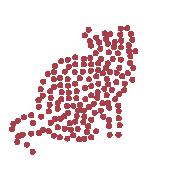
\includegraphics[width=.17\linewidth]{figures/monge-shape-mccann-interpolation/particles-t025.pdf} &

\includegraphics[width=.17\linewidth]{figures/monge-shape-mccann-interpolation/particles-t050.pdf} &
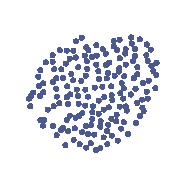
\includegraphics[width=.17\linewidth]{figures/monge-shape-mccann-interpolation/particles-t075.pdf} &

\includegraphics[width=.17\linewidth]{figures/monge-shape-mccann-interpolation/particles-t100.pdf} \\[-.1em]
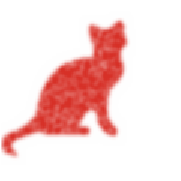
\includegraphics[width=.17\linewidth]{figures/monge-shape-mccann-interpolation/density-t000.pdf} &
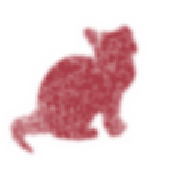
\includegraphics[width=.17\linewidth]{figures/monge-shape-mccann-interpolation/density-t025.pdf} &

\includegraphics[width=.17\linewidth]{figures/monge-shape-mccann-interpolation/density-t050.pdf} &

\includegraphics[width=.17\linewidth]{figures/monge-shape-mccann-interpolation/density-t075.pdf} &

\includegraphics[width=.17\linewidth]{figures/monge-shape-mccann-interpolation/density-t100.pdf}
\end{tabular}
\caption{McCann displacement interpolation between a cat silhouette and a heart silhouette. The first row displays transported particles along $T_t(x)=(1-t)x+tT(x)$; the second row shows kernel-smoothed densities computed from a larger cloud, making the evolving support easier to read.}
\label{fig:monge-shape-mccann-interpolation}
\end{figure}

\begin{prop}[Knothe--Rosenblatt triangular rearrangement]\label{prop-knothe-rosenblatt}
	Let $\al,\be\in\Mm_+^1(\RR^d)$. Assume, for simplicity, that the first marginal of $\al$ and the one-dimensional conditional laws of $\al$ used below are atomless, and that regular conditional distributions are fixed. There is a triangular map
	\[
		\T(x_1,\ldots,x_d)
		=
		(\T_1(x_1),\T_2(x_1,x_2),\ldots,\T_d(x_1,\ldots,x_d))
	\]
	such that $\T_\sharp\al=\be$ and, for each $k$, the function $x_k\mapsto\T_k(x_1,\ldots,x_k)$ is nondecreasing for $\al$-almost every value of $(x_1,\ldots,x_{k-1})$.
\end{prop}
\begin{proof}
	The construction is recursive. For $k=1$, let $\T_1$ be the monotone rearrangement between the first marginal of $\al$ and the first marginal of $\be$. Suppose that $\T_1,\ldots,\T_{k-1}$ have already been constructed. Write $x_{<k}=(x_1,\ldots,x_{k-1})$ and $\T_{<k}=(\T_1,\ldots,\T_{k-1})$. By induction, $(\T_{<k})_\sharp\al_{<k}=\be_{<k}$, where $\al_{<k}$ and $\be_{<k}$ are the first $(k-1)$-coordinate marginals. Let $\al^k_{x_{<k}}$ and $\be^k_{y_{<k}}$ be regular conditional laws of the $k$-th coordinate given the previous coordinates. Define $\T_k(x_{<k},\cdot)$ as the one-dimensional monotone rearrangement from $\al^k_{x_{<k}}$ to $\be^k_{\T_{<k}(x_{<k})}$.

	The map $\T_k(x_{<k},\cdot)$ is nondecreasing by the one-dimensional rearrangement theorem. The chain rule for disintegrations then shows that, after step $k$, the first $k$ coordinates of $\T_\sharp\al$ have the same law as the first $k$ coordinates of $\be$. At $k=d$ this gives $\T_\sharp\al=\be$. Target atoms are handled by generalized quantiles. If a source conditional law has atoms that must be split, the same recursive construction defines a triangular Markov kernel rather than a deterministic map.
\end{proof}

This construction transports successively along coordinate axes and is therefore often called axis-wise transport. It depends on the chosen ordering of coordinates and is not generally optimal for the quadratic cost. It is nevertheless a useful limiting object: Brenier maps for increasingly anisotropic quadratic costs converge to triangular rearrangements under suitable assumptions~\cite{carlier2010knothe}.

%%%%%%%%%%%%%%%%%%%%%%%%%%%%%%%%%%%%%%%%%%%%%%%%%%%%%%%%%%%%%%%%%%%%%%%%%%%
\subsection{Vector Quantiles and Linearized Transport}
\label{sec-vector-quantiles-linearized-transport}

The one-dimensional quantile function represents a probability measure by the monotone map sending a fixed reference law to it. In dimension $d>1$, Brenier's theorem gives the analogous construction after choosing a reference probability $\rho_0$, typically the uniform law on a convex body or a standard Gaussian.

\paragraph{Vector quantiles.}

Assume that the reference law $\rho_0$ is absolutely continuous. For a target law $\mu$ with finite second moment, its vector quantile relative to $\rho_0$ is the Brenier map
\[
	\T_\mu=\nabla\phi_\mu,
	\qquad
	(\T_\mu)_\sharp\rho_0=\mu,
\]
or equivalently the solution of
\[
	\min_{\T_\sharp\rho_0=\mu}
	\int \norm{x-\T(x)}^2\d\rho_0(x).
\]
This construction is canonical only after fixing $\rho_0$: changing the reference law changes the coordinates used to represent $\mu$. Vector quantile regression uses the same idea conditionally, replacing scalar conditional quantiles by conditional Brenier maps and thereby encoding multivariate ranks and depths~\cite{carlier2016vector}.

\paragraph{Linearized Wasserstein coordinates.}

The same reference measure leads to the linearized OT embedding
\[
	\mu\longmapsto \T_\mu-\Id\in L^2(\rho_0;\RR^d).
\]
Distances between embedded maps are not equal to Wasserstein distances in general, but they provide a useful tangent-space approximation. In one dimension the construction is exact because quantile functions give the isometry~\eqref{eq-wass-cumul}. Section~\ref{sec-linear-ot} uses this reference-map viewpoint to build fast linearized barycenters: for varying weights, one averages maps in $L^2(\rho_0)$ and pushes $\rho_0$ forward by the averaged map. Figure~\ref{fig:monge-linearized-transport-coordinates} visualizes these coordinates as displacement fields from a fixed disk reference.

\begin{figure}[H]
\centering
\begin{tabular}{@{}cc@{}}
\small red target mixture & \small purple target mixture \\[-.15em]
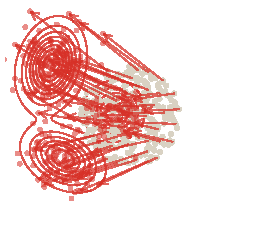
\includegraphics[width=.43\linewidth]{figures/monge-linearized-transport-coordinates/red-mixture.pdf} &
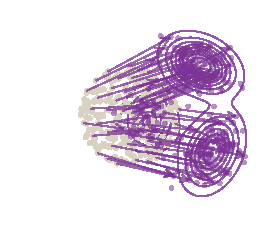
\includegraphics[width=.43\linewidth]{figures/monge-linearized-transport-coordinates/purple-mixture.pdf}
\end{tabular}
\caption{Linearized transport coordinates around a fixed disk reference. The gray points sample the reference law, colored contours show the target density, and the arrows display a farthest-point subsample of the barycentric projection $T_\mu-\Id$ of the quadratic OT map. The full OT map is computed on a denser cloud than the arrows shown here.}
\label{fig:monge-linearized-transport-coordinates}
\end{figure}

%%%%%%%%%%%%%%%%%%%%%%%%%%%%%%%%%%%%%%%%%%%%%%%%%%%%%%%%%%%%%%%%%%%%%%%%%%%
\subsection{Gaussian Measures and the Bures Metric}
\label{sec-gaussian-bures}

Gaussian measures form the most important finite-dimensional family preserved by quadratic optimal transport. The mean moves linearly, while the covariance follows the Bures--Wasserstein geometry of positive semidefinite matrices.

\paragraph{One-dimensional Gaussians.}

Let $\al=\Gaussian(m_\al,s_\al^2)$ and $\be=\Gaussian(m_\be,s_\be^2)$ be two nondegenerate Gaussians on $\RR$. Then
\[
	\T(x)=\frac{s_\be}{s_\al}(x-m_\al)+m_\be
\]
satisfies $\T_\sharp\al=\be$. It is the derivative of the convex function
\[
	\phi(x)=\frac{s_\be}{2s_\al}(x-m_\al)^2+m_\be x,
\]
so Brenier's theorem shows that it is the optimal quadratic transport. The associated distance is
\[
	\Wass_2(\al,\be)^2
	=
	\int_\RR\left(\frac{s_\be}{s_\al}(x-m_\al)+m_\be-x\right)^2\d\al(x)
	=
	(m_\al-m_\be)^2+(s_\al-s_\be)^2.
\]
The formula extends by continuity to Dirac masses, although the affine Monge map itself only pushes a Dirac source to another Dirac. Thus the OT geometry of one-dimensional Gaussians is the Euclidean geometry of the half-plane $(m,s)\in\RR\times\RR_+$. This contrasts with KL geometry, where singular Gaussians are infinitely distant.

\paragraph{Multivariate Gaussians.}

If
\eql{\label{eq-gauss-pf}
	\al=\Gaussian(\mean_\al,\cov_\al),
	\qquad
	\be=\Gaussian(\mean_\be,\cov_\be),
	\qquad
	\T(x)=\mean_\be+A(x-\mean_\al),
}
then $\T$ is the gradient of the convex quadratic potential $\phi(x)=\dotp{\mean_\be}{x}+\dotp{A(x-\mean_\al)}{x-\mean_\al}/2$ if and only if $A$ is symmetric positive semidefinite.

\begin{prop}[Affine push-forward of Gaussians]\label{prop-gaussian-affine-push-forward}
	One has $\T_\sharp\al=\be$ if and only if
	\eql{\label{eq-gauss-covariance-pushforward}
		A\cov_\al A^\top=\cov_\be.
	}
\end{prop}
\begin{proof}
	An affine function maps a Gaussian to a Gaussian, so the law of $\T(X)$ is determined by its mean and covariance. If $X\sim\al$ and $Y=\T(X)$, then
	\[
		\EE(Y)=\mean_\be+A\EE(X-\mean_\al)=\mean_\be,
	\]
	and
	\[
		\EE((Y-\mean_\be)(Y-\mean_\be)^\top)
		=
		A\EE((X-\mean_\al)(X-\mean_\al)^\top)A^\top
		=
		A\cov_\al A^\top.
	\]
	Thus $A\cov_\al A^\top=\cov_\be$ is necessary and sufficient for $Y$ to have the same mean and covariance as $\be$.
\end{proof}

The covariance equation is quadratic in $A$. Under the symmetry constraint imposed by Brenier's theorem, it becomes $A\cov_\al A=\cov_\be$. The next proposition solves this equation and computes the resulting transport cost.

\begin{prop}[Gaussian $\Wass_2$ formula and Bures covariance term]\label{prop-gaussian-w2-bures}
	Assume that $\cov_\al$ and $\cov_\be$ are positive definite. The unique symmetric positive-definite solution of
	\[
		A\cov_\al A=\cov_\be
	\]
	is
	\eql{\label{eq-bures-map}
		A=
		\cov_\al^{-1/2}
		\pa{\cov_\al^{1/2}\cov_\be\cov_\al^{1/2}}^{1/2}
		\cov_\al^{-1/2}.
	}
	The affine map $\T(x)=\mean_\be+A(x-\mean_\al)$ is the optimal quadratic-cost transport from $\Gaussian(\mean_\al,\cov_\al)$ to $\Gaussian(\mean_\be,\cov_\be)$, and
	\eql{\label{eq-dist-gauss}
		\Wass_2(\al,\be)^2
		=
		\norm{\mean_\al-\mean_\be}^2+\Bb(\cov_\al,\cov_\be)^2,
	}
	where
	\eql{\label{eq-bure-defn}
		\Bb(\cov_\al,\cov_\be)^2
		\eqdef
		\tr\pa{\cov_\al+\cov_\be-2(\cov_\al^{1/2}\cov_\be\cov_\al^{1/2})^{1/2}}.
	}
\end{prop}
\begin{proof}
	Multiplying $A\cov_\al A=\cov_\be$ on the left and right by $\cov_\al^{1/2}$ gives
	\[
		(\cov_\al^{1/2}A\cov_\al^{1/2})^2
		=
		\cov_\al^{1/2}\cov_\be\cov_\al^{1/2}.
	\]
	Since $A$ is symmetric positive, $\cov_\al^{1/2}A\cov_\al^{1/2}$ is symmetric positive and is therefore the unique positive square root of the right-hand side. Conversely, the matrix in~\eqref{eq-bures-map} is symmetric positive and satisfies the covariance equation.

	By Proposition~\ref{prop-gaussian-affine-push-forward}, this affine map pushes $\al$ to $\be$. It is the gradient of a convex quadratic potential, so Brenier's theorem implies optimality. If $X\sim\al$, then
	\begin{align*}
		\EE\norm{X-\T(X)}^2
		&=
		\norm{\mean_\al-\mean_\be}^2
		+
		\EE\norm{(I-A)(X-\mean_\al)}^2 \\
		&=
		\norm{\mean_\al-\mean_\be}^2
		+
		\tr((I-A)\cov_\al(I-A)^\top) \\
		&=
		\norm{\mean_\al-\mean_\be}^2
		+
		\tr(\cov_\al)+\tr(A\cov_\al A)-2\tr(A\cov_\al) \\
		&=
		\norm{\mean_\al-\mean_\be}^2
		+
		\tr(\cov_\al)+\tr(\cov_\be)
		-2\tr((\cov_\al^{1/2}\cov_\be\cov_\al^{1/2})^{1/2}),
	\end{align*}
	which is the desired expression. The formula for singular covariance matrices follows by adding $\eta I$ and letting $\eta\downarrow0$.
\end{proof}

The covariance term $\Bb$ is the Bures--Wasserstein metric on positive semidefinite matrices~\cite{bures1969extension,gelbrich1990formula,bhatia2018bures}. It separates the Euclidean displacement of the mean from the intrinsic transport geometry of covariance ellipsoids.

\begin{prop}[Metric and convexity properties of the Bures term]\label{prop-bures-metric-convex}
	The function $\Bb$ is a distance on positive semidefinite covariance matrices. Moreover, $\Bb^2$ is jointly convex: for $t\in[0,1]$,
	\[
		\Bb^2((1-t)\Sigma_0+t\Sigma_1,(1-t)\Lambda_0+t\Lambda_1)
		\leq
		(1-t)\Bb^2(\Sigma_0,\Lambda_0)+t\Bb^2(\Sigma_1,\Lambda_1).
	\]
\end{prop}
\begin{proof}
	The key identity is the Procrustes representation
	\[
		\Bb^2(\Sigma,\Lambda)
		=
		\min_{Q^\top Q=I}\norm{\Sigma^{1/2}-\Lambda^{1/2}Q}_F^2.
	\]
	Indeed, expanding the square gives $\tr\Sigma+\tr\Lambda-2\max_{Q^\top Q=I}\tr(\Sigma^{1/2}Q^\top\Lambda^{1/2})$, and the orthogonal Procrustes formula identifies the maximum with $\tr((\Sigma^{1/2}\Lambda\Sigma^{1/2})^{1/2})$. Symmetry, positivity and separation follow immediately from this representation. The triangle inequality follows by choosing two almost optimal orthogonal matrices $Q_1,Q_2$ and writing
	\[
		\norm{\Sigma^{1/2}-\Gamma^{1/2}Q_2Q_1}_F
		\leq
		\norm{\Sigma^{1/2}-\Lambda^{1/2}Q_1}_F
		+
		\norm{\Lambda^{1/2}-\Gamma^{1/2}Q_2}_F.
	\]
	Letting the two choices become optimal proves the metric property.

	For convexity, use the equivalent factor formulation
	\[
		\Bb^2(\Sigma,\Lambda)
		=
		\min_{UU^\top=\Sigma,\thinspace VV^\top=\Lambda}\norm{U-V}_F^2.
	\]
	Choose nearly optimal factors $(U_0,V_0)$ and $(U_1,V_1)$ for the two pairs, and define block factors
	\[
		U_t=[\sqrt{1-t}\,U_0,\sqrt t\,U_1],
		\qquad
		V_t=[\sqrt{1-t}\,V_0,\sqrt t\,V_1].
	\]
	Then $U_tU_t^\top=(1-t)\Sigma_0+t\Sigma_1$ and $V_tV_t^\top=(1-t)\Lambda_0+t\Lambda_1$, while
	\[
		\norm{U_t-V_t}_F^2
		=
		(1-t)\norm{U_0-V_0}_F^2+t\norm{U_1-V_1}_F^2.
	\]
	Taking the infimum over the initial factors proves joint convexity.
\end{proof}

\begin{rem}[Diagonal covariances and Hellinger geometry]
	If $\cov_\al=\diag(r_i)_i$ and $\cov_\be=\diag(s_i)_i$ are diagonal, the Bures metric reduces to the Euclidean distance between square roots,
	\[
		\Bb(\cov_\al,\cov_\be)=\norm{\sqrt r-\sqrt s}_2.
	\]
	This is the finite-dimensional Hellinger geometry on the nonnegative covariance coordinates: variances are compared after the amplitude change of variables $r_i\mapsto\sqrt{r_i}$.
\end{rem}
